\documentclass[12pt,conference]{IEEEtran}
%\documentclass[letterpaper,twocolumn,10pt]{article}

\usepackage{graphicx}
\usepackage{url}
\usepackage[usenames]{color}
\usepackage{listings}
\usepackage{wrapfig}
\usepackage{dirtytalk}
\usepackage[caption=false]{subfig}
\usepackage[export]{adjustbox}

\newcommand{\citationneeded}{\textsuperscript{\textit{[CitationNeeded]}}}

%------------------------------------------------------------------------- 
% take the % away on next line to produce the final camera-ready version 
\pagestyle{empty}
\pagenumbering{arabic}
%------------------------------------------------------------------------- 
\begin{document}

\title{Continuous Integration in Software Management}


%for single author (just remove % characters)
\author{
{\rm Gautam Kumar, Prof. David Socha}\\
Computing and Software Systems\\
University of Washington, Bothell\\
\{gautamk,socha\}@uw.edu
} % end author

\maketitle
\thispagestyle{empty}


\section*{Abstract}
Continuous Integration, a practice where developers integrate 
frequently \cite{stahl_modeling_2014} is considered an integral part of Agile 
development. CI is often thought to be a safety net that prevents developers from deploying broken code to production. 

A similar process and ideology of continual improvement and integration can be applied to Software Management, the art and science of planning and leading software projects \cite{stellman_applied_2005}.

This paper attempts to explore the process of creating such an integration practice within an Organisation.

\subsubsection*{Keywords}

Software Management, Agile development, Continuous Integration

\section*{Introduction}

Martin Fowler in his seminal article \cite{fowler_continuous_2006} on Continuous Integration (CI) describes it as a practice where members of a team integrate their work frequently and each integration is verified by an automated build to detect problems quickly.

In the context described above integration is the process of combining the work of all the developers of a project into a cohesive software. On the other hand if considered generically, Integration can be thought of as a practice of combining the work of multiple people and verifying its correctness. Using a similar collective, Continuous integration could be the process of merging the work of multiple people after specific events or set periods of time.

TODO Expand


\section*{Continuous Improvement}

The American Society of Quality define Continuous Improvement to be 
\say{The ongoing improvement of products, services or processes through incremental and breakthrough improvements.} \cite{american_society_for_quality_continuous_????}

Continuous Improvement as a concept has existed for a long time. We can find mentions to continuous Improvement in texts dating back to the mid-19th century \cite{schroeder_americas_????}. 

During the Industrial revolution of the mid-19th century workers were often trained not to think but rather just perform just their task. Thus the task of thinking was effectively cut off from the task of doing, which lead to the thinkers not understanding the practical restrictions of the real world and the increasing complexity of the systems \cite{schroeder_americas_????}. The same concept applies even today with software systems, computers have taken on the role of workers while humans have moved on to the task of thinking.

This separation of thinkers from the practical implications of real world lead to the development of Continuous improvement which emphasizes a continuous stream incremental innovation \cite{bessant_rediscovering_1994}.

Continuous improvement is one of the primary pre-requisites for continuous integration. A stable, unmaintained project does not change and thus has no need for a continual process of integration. We assume here that any changes introduced into a project is designed to improve the project in some way. There are situations where changes don't necessarily improve the project such as when malicious code in secretly introduced. 


\section*{Continuous Integration}

\subsection*{History}

The term continuous integration was first used by Grady Booch in his 1994 book \cite{booch_object-oriented_1994}. Booch refers to continuous integration as a micro process which produces many internal releases. He also mentions that testing should also be conducted as a continuous activity during the development process.

Kent Beck and Ron Jeffries, the inventors of Extreme Programming(XP), wrote about implementing continuous integration in their book on XP \cite{astesiano_fundamental_1998}. Beck and Jeffries had worked together on building a payroll application for the Chrysler corporation and pioneered the process of XP during their time working on the Chrysler Comprehensive Compensation System (C3). Beck and Jeffries implemented the CI process within the C3 development team as a method to escape integration hell while also promoting the concept that all developers must work on the most recent release of the system \cite{cunningham_cunningham_2011}.

\subsection*{Complexity}
Continuous improvement incentivizes a structure where anyone in the organisation who possess  a basic skill set can contribute to the implementation of solutions for a common problem set \cite{bessant_rediscovering_1994}. Such a process brings along with it an explosion of ideas and as some of those ideas implemented complexity increases drastically. Such an increase in complexity eventually leads to either the quality or velocity of development to decline \cite{zaytsev_increasing_2013}. 

Continuous integration thus evolved as a mechanism to manage the risk associated with complex software systems \cite{zaytsev_increasing_2013} and  attempts to provide a safety net \cite{fowler_continuous_2006} to developers. 

Though continuous integration doesn't actually fix bugs, it offers a lot of benefits which help in improving the overall quality of the project such as Improved communication, Project predictability and increased developer productivity \cite{sta_ahl_experienced_2013}. So Continuous integration in many ways can be considered a modern method of complexity control \cite{beck_extreme_2000}.

\begin{figure*}[Ht!]
  \centering
  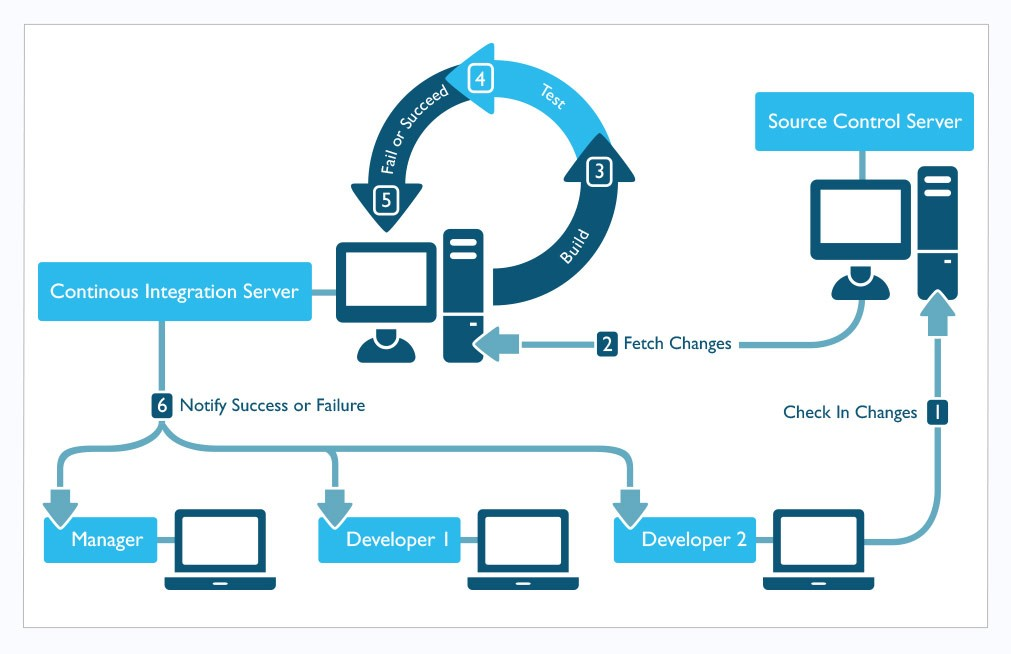
\includegraphics[height=3in]{ci_process}
  \caption{A typical CI process, source: \cite{cois_continuous_2015}}
  \label{leakyabstraction}
\end{figure*}



\section*{Software Management and Continuous Integration}

The inherent complexity in software management is best described by the law of leaky abstractions \cite{spolsky_law_2002} which states that all non-trivial abstractions leak to some degree. 

\subsection*{The Law of leaky abstractions}

An abstraction in the context of computers and software refers to a mechanism that tries to hide the complexity of the underlying system while still offering a useful interface to interact effectively with the underlying system. Abstractions are meant to simplify the process of interacting with an inherently complex system by hiding away certain irrelevant details.

Though abstractions vastly simplify interactions with a complex system, the abstractions are still limited by the capabilities of underlying system and  thus some serious failures always trickle up through abstractions and surprise the user in unexpected ways. Fig \ref{leakyabstraction} describes such a trickle from hardware all the way to the application level.

\begin{figure*}
  \centering
  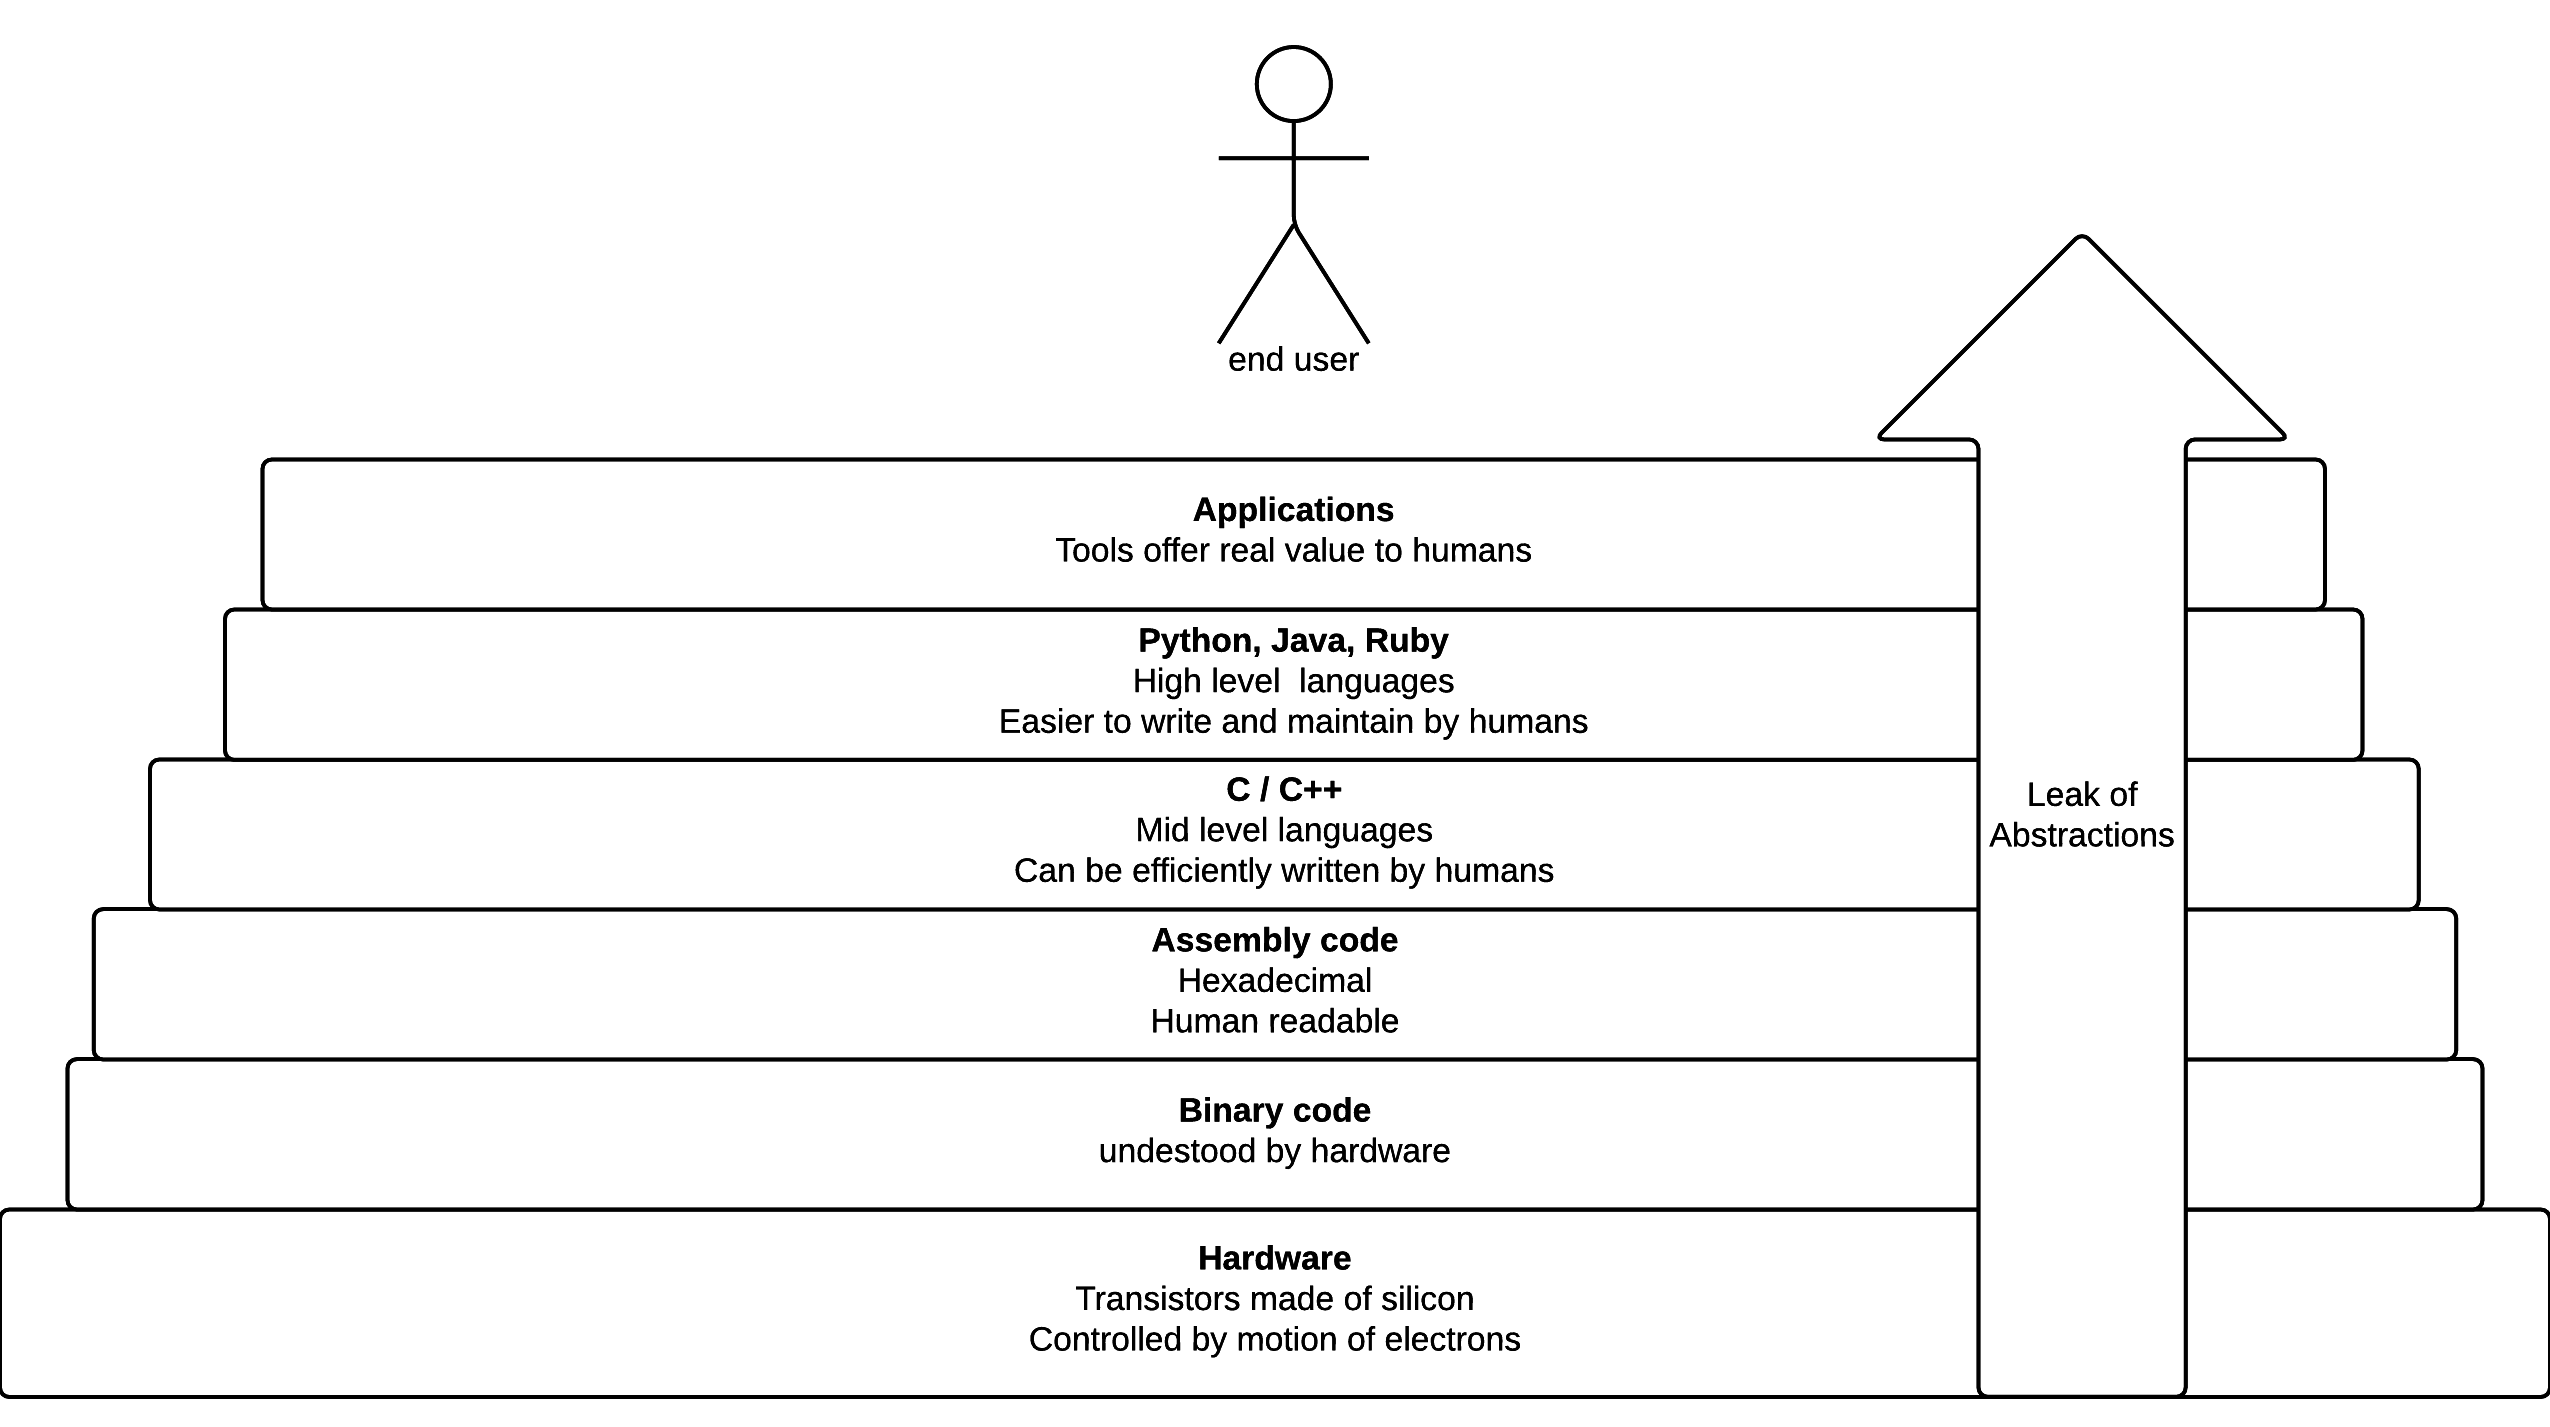
\includegraphics[height=4in]{leakyabstraction}
  \caption{The law of leaky abstraction: All non-trivial abstractions, to some degree, are leaky.}
  \label{leakyabstraction}
\end{figure*}

A classic example of leaky abstractions would be Operating Systems. On the windows operating system any failure in the underlying hardware or its drivers can potentially lead to a BSOD (Blue screen of death) in which the computer displays a cryptic message on a blue screen and prompts the user for action. Though BSOD is a rare occurrence under normal operating conditions, its appearance often perplexes an average user who is unable to make a decision on the next course of action \cite{rosenberg_law_2007}. 

\subsection*{Abstractions in Software Management}

Software Management as a subset of Project management is primarily concerned with balancing the needs of stakeholders with the abilities of developers to deliver value.

Software management practices abstract away the inner workings processes in the organisation. For example Agile methodologies such as Scrum and Kanban are an abstraction which uses best practices from Time management, Team communication, Performance management and Theory of constraints to derive value from developers collaborating within a team. 

Another example of abstraction in Software management in teams would be embracing diversity which is an abstraction over Psychology and Economics to help teams take varied view points on any particular problem. 

\subsection*{Cynefin perspective}

The Cynefin model describes the relationship between the ability to determine causality in a situation and the way people respond to said situation. The model describes four states. The obvious state where cause and effect are easy to determine so people can sense, categorise and respond. The complicated state where the cause is not immediately apparent but can easily be determined by sensing, analysing and responding. The complex state where it neither the cause nor the effect is immediately apparent but we can run experiments to verify our direction so we probe sense and respond. The chaotic state where the system is not stable and we cannot wait to determine the state of the system so we act, sense and respond. Finally we have a state where it is not possible to determine the domain of the system
Fig \ref{cynefin} describes the various states of the cynefin model in a easy to visualize manner.

When considered from the perspective of the Cynefin model \cite{snowden_cynefin_????}, the relationship between software management processes and the people in the organisation can range from complex to outright chaotic. For example in an organisation where many people have experience working in an agile environment working within the bound of the organisation's implementation of agile can be a complex task for an individual. On the other hand when an organisation moves from waterfall towards agile, people in the organisation have a chaotic relationship with the new software management process and struggle to adapt to the new way of thinking. Agile software development thrives just at the edge of chaos and its easy to slip into a chaotic state when trying to transition from other software management methodologies \cite{kautz_just_2008}. 


\begin{figure}[hbtp]
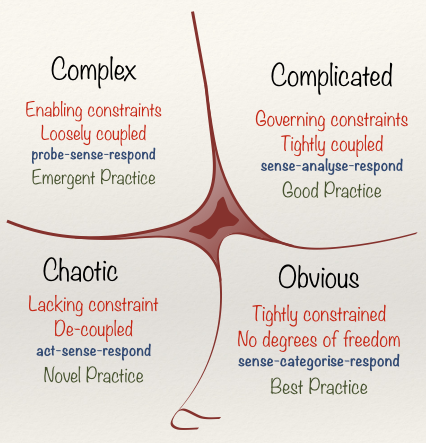
\includegraphics[scale=0.55]{cynefin.png}
\caption{The Cynefin model, The states on the left are un-ordered sates where causality cannot be determined and the states on the right are ordered where the system is highly constrained so causality is either obvious or easy to determine. The central dark area refers to un-determinable state when the state of the system cannot be determined by any reasonable means  \cite{snowden_leaders_2007}}
\label{cynefin}
\end{figure}

\subsection*{CI in Software Management}

Software management is in essence a process which tries to abstract away the chaos of managing an inherently complex task with the help of developers in an ever-evolving environment. As with any non trivial abstraction, software management is leaky and implementing continuous integration into Software management practices could potentially offer benefits similar to software development.


\section*{Scope of Software Management}

The software management process can include areas of management which traditionally come under the purview of Project management such as people management and customer relations. Including these factors into the software management process is however crucial to the overall goal of efficient and effective management of the software process to enable developers to build products that deliver value.

Some potential areas which might come under the purview of software management are

\begin{itemize}

\item People Management
\begin{itemize}
\item Hiring
\item Culture
\item Expectations
\item Organisation structure
\item Diversity
\end{itemize}

\item Project management
\begin{itemize}
\item Requirements gathering
\item Technical choices
\item Project priorities
\item Team selection
\end{itemize}

\item Product management
\begin{itemize}
\item Market analysis
\item Solving the right problem
\end{itemize}

\item Process management
\end{itemize}


\section*{Continuous integration in people management}

In the paper we limit the scope of implementing Continuous Integration in the software management process within people management and its potential benefits.

Continuous integration has been well defined from the software development perspective, definitions from the perspective of Software Management on the other hand are quite sparse. 

Continuous integration is best implemented in an organisation where a significant emphasis is placed on continuous improvement and failure is considered a part of the learning process \cite{edmondson_strategies_2011}.

The easiest area to define Continuous Integration within the scope of Software management would be people management. Continuous Integration in terms of People management could be thought of as a way to verify that the everyone in the organisation is working towards a common goal.


\subsection*{Relation to software management}

An organisation's products and the value derived from them are built by people in the organisation. In a software organisation the primary product is software so managing the people who build software would come under the purview of software management. 

\subsection*{Implementing continuous integration}

Continuous Integration and improvement are by their nature an iterative process thus implementing them within the context of software management requires the management team to follow a disciplined process of continuous evaluation and an evolution.

\subsection*{On boarding new hires}

As an example we consider on boarding new hires to highlight ways to introduce continuous integration into an organisation.

\subsubsection*{Adoption}

The initial adoption process of any new software management model would be significantly different from integrating new team members into an existing model. For example, some the factors which affect the success of adopting Agile methodologies in an organisation are 
Customer collaboration, satisfaction and commitment, Communication and negotiation skills of the team and Cultural factors \cite{misra_identifying_2009}.

These success factors differ when bringing in new team members. For example a team member fresh out of college might adapt to an existing process at an organisation with ease while a seasoned developer who is loyal to the waterfall model might have a hard time adapting to the rapid pace of an agile organisation. 

As teams being to understand the expectations of their customers and their organisations the previously defined software process evolves thus as time goes on each team / organisation starts building a unique variation of the agile process.

In this context initial adoption is usually the easiest task as the whole team is collectively working towards making sure that Agile adoption succeeds. Adoption by new team members on the other hand depends on the new team member, the Software management team and the culture of the organisation.

It is the responsibility of the software management team to enable new developers to adopt and adapt to the unique process of the dev team they are going to be working with.

\begin{figure}[t]
\centering
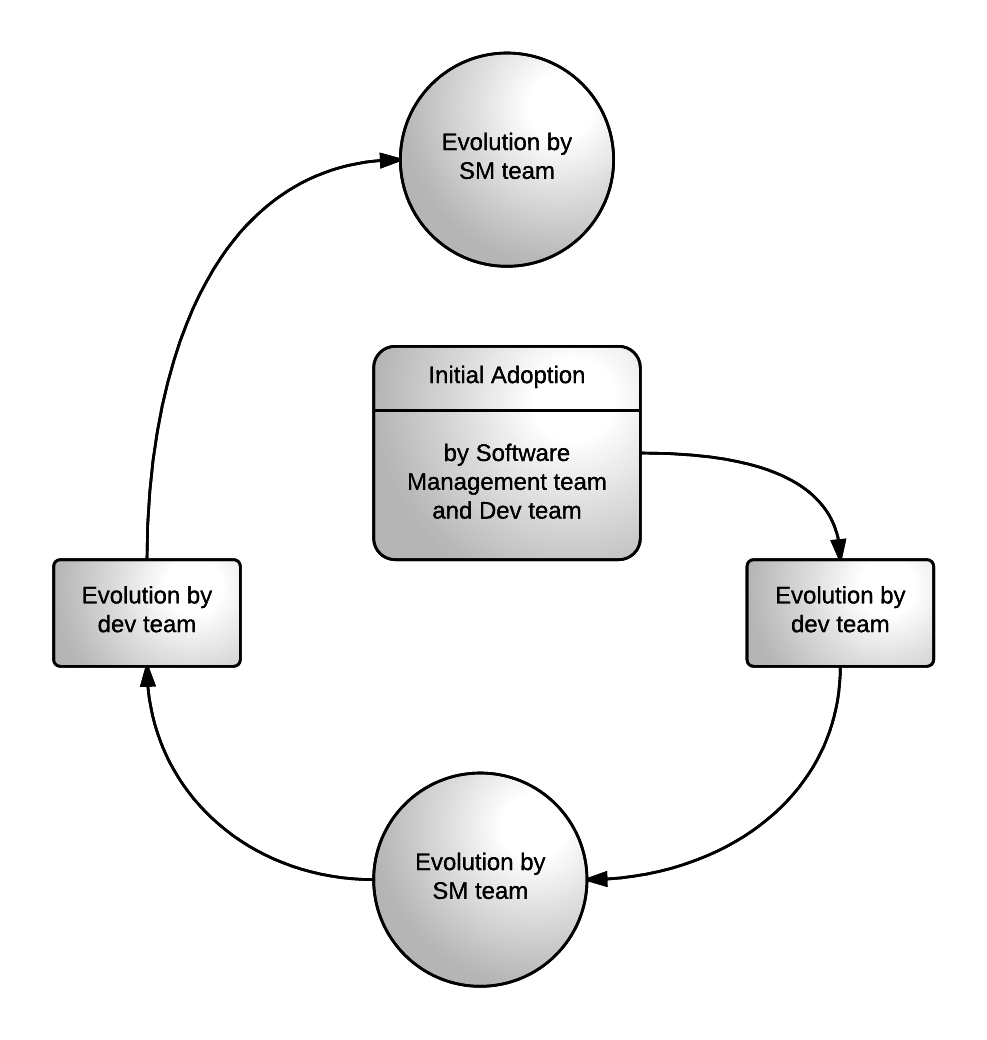
\includegraphics[width=0.4\textwidth]{sm_dev_team_process_evolution.png}
\caption{The Software management team has to evolve the adoption process as the dev team deviates from the initial Software developement model}
\end{figure}



\subsubsection*{Success criteria} The software management team needs to have a clear and evolving success criteria which monitors each new hire and how well they are able to adapt to their new teams. This differs from Definition of Done (DoD) based on the fact that DoD is merely a set of activities which need to be performed to get the user story to a shippable state while Success criteria is a broader set of expectations from the candidate which are recorded based on subjective observations. 

Some of the metrics to measure under success criteria could be Team communication, Knowledge sharing \cite{cabrera_fostering_2005}, Productivity acceleration \cite{grote_making_2011} and Empathy \cite{seppala_hard_2014}.

Success criteria in this case could potentially be defined as "After an initial introductory period, A new employee has learnt `X` new things from their team members and their productivity has increased by a factor of `Y`"

\subsubsection*{Continuous Integration}
As an example continuous integration from the perspective of on-boarding new hires can potentially be implemented as an internal process which evaluates the effectiveness of the on boarding process with both the team, the new member and the management to evaluate value of the on boarding process, effectiveness of its implementation and any potential flaws or breaks in its implementation. 

Any implementation of the on boarding process could potentially break due to changes from either the dev team or the people management team. For example the dev team might introduce a new method of code review but this code review technique might be missing from the orientation packet for new hires. The continuous integration process for evaluating new hires could potentially catch this so that it can be corrected quickly.


\section*{Summary}

In this paper we describe the how software management is a complex task using the Cynefin model and the law of leaky abstraction. We also describe why continuous integration can help discover flaws in the process early with a case study about on-boarding new hires.

\bibliographystyle{plain}
\bibliography{css566_software_management}

\end{document}

